\chapter{放大电路中的反馈}
在电路中引入负反馈后,也可以使得电路保持稳定,并取得一些其他意想不到的效果。
\section{反馈的基本概念与分类}
\subsection{反馈的基本概念}
\textbf{反馈}是指电路的输出量的一部分或者全部通过一定的电路形式作用到输入回路,以影响输入量。
\begin{figure}[htb]
    \centering
    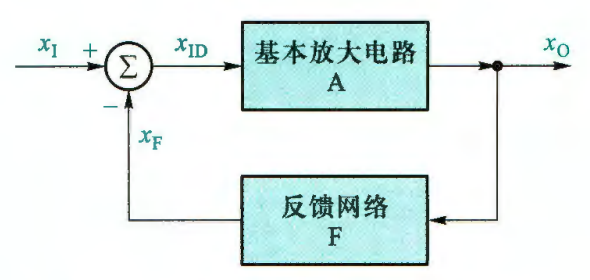
\includegraphics[width=0.5\linewidth]{pic/反馈.png}
    \caption{反馈放大电路的方框图\cite{康华光}\label{反馈}}
\end{figure}

其中$x_{\mathrm{I}}$表示输入信号,$x_{\mathrm{O}}$表示输出信号,$x_{\mathrm{ID}}$表示净输入信号,$x_{\mathrm{F}}$表示反馈信号。而\textbf{基本放大电路增益}为$A=x_{\mathrm{O}}/x_{\mathrm{ID}}$,\textbf{反馈系数}$F=x_{\mathrm{F}}/x_{\mathrm{O}}$。

\subsection{基本反馈的分类与判断}\label{基本反馈的分类与判断}
\subsubsection{一、开环与闭环}
若没有反馈网络,称为\textbf{开环}\index{K!开环},而如果存在反馈网络,则称为\textbf{闭环}\index{B!闭环}。

判断电路中有无反馈只需要看有无将输出回路和输入回路相连接的通路即可。

\subsubsection{二、级内反馈和级间反馈}
每级各自存在的反馈就是\textbf{级内反馈}\index{F!反馈!级内反馈},跨级的反馈就是\textbf{级间反馈}\index{F!反馈!级间反馈}。

\subsubsection{三、直流反馈和交流反馈}
存在于直流通路中的反馈称为\textbf{直流反馈}\index{F!反馈!直流反馈},而存在于交流通路中的反馈称为\textbf{交流反馈}\index{F!反馈!交流反馈}。

\subsubsection{四、正反馈和负反馈}
使净输入量变大的反馈称为\textbf{正反馈}\index{F!反馈!正反馈},使净输入量变小的反馈称为\textbf{负反馈}\index{F!反馈!负反馈}。

常用方法为“瞬时极性法”:首先假设瞬时极性增加,用(+)标出,然后沿着信号传输的路径判断有关节点电压的瞬时值。若增强输入信号就为正反馈,否则为负反馈。

\begin{figure}[htb]
    \centering
    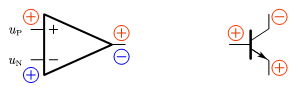
\includegraphics[width=0.5\linewidth]{pic/反馈极性的判断.png}
    \caption{常用元件反馈极性的判断\label{反馈极性的判断}}
\end{figure}

\section{负反馈放大电路的四种组态及判断}
除了\ref{基本反馈的分类与判断}小节中提到的四种分类方法,反馈电路还可以分为串联/并联反馈和电压/电流反馈,而这两种分类通常是对\textbf{交流负反馈}放大电路而言的,非常重要,因此独成一节。

\subsection{串联反馈和并联反馈}
根据在反馈网络的输出端口和基本放大电路的输入端口的连接方式来判定。凡是反馈网络的输出端口与基本放大电路的输入端口串联连接的,为\textbf{串联反馈}\index{F!反馈!串联反馈};凡是反馈网络的输出端口与基本放大电路的输入端口并联连接的,为\textbf{并联反馈}\index{F!反馈!并联反馈}。

由定义可以知道,串联/并联反馈反映的是输入信号和反馈信号的叠加方式,而两个可以叠加的信号一定具有相同的量纲。因此,如果两个信号都是电压信号,则只能进行“串联”;如果两个信号都是电流信号,则只能进行“并联”(类比串联分压,并联分流)。

由上面的讨论可以得到一个快捷的判断方式:当反馈信号与输入信号接入不同端时,二者无法进行电流的叠加,叠加的是电压信号,是串联反馈;而当反馈信号与输入信号接入相同端时,可以进行电流的叠加,是并联反馈。

\begin{figure}[htb]
    \centering
    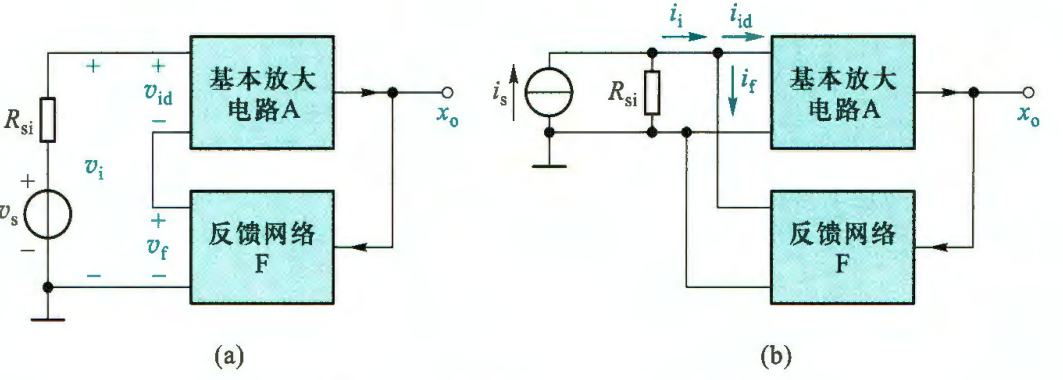
\includegraphics[width=0.75\linewidth]{pic/串联反馈和并联反馈.png}
    \caption{串联反馈和并联反馈(a)串联反馈(b)并联反馈\cite{康华光}\label{串联反馈和并联反馈}}
\end{figure}

\subsection{电压反馈和电流反馈}
根据在反馈网络的输入端口和基本放大电路的输出端口的取样对象来判定。

当反馈信号和输出电压成比例,为\textbf{电压反馈}\index{F!反馈!电压反馈};若与电流成比例,为\textbf{电流反馈}\index{F!反馈!电流反馈}。

当网络存在负反馈时,必定是电压反馈和电流反馈其中的一种。因此有一种特殊的判定方法——“输出短路法”。当输出电压$v_\mathrm{o}=0$时,反馈信号也不存在了,则反馈信号与输出电压成比例,为电压反馈,否则为电流反馈。

\begin{figure}[htb]
    \centering
    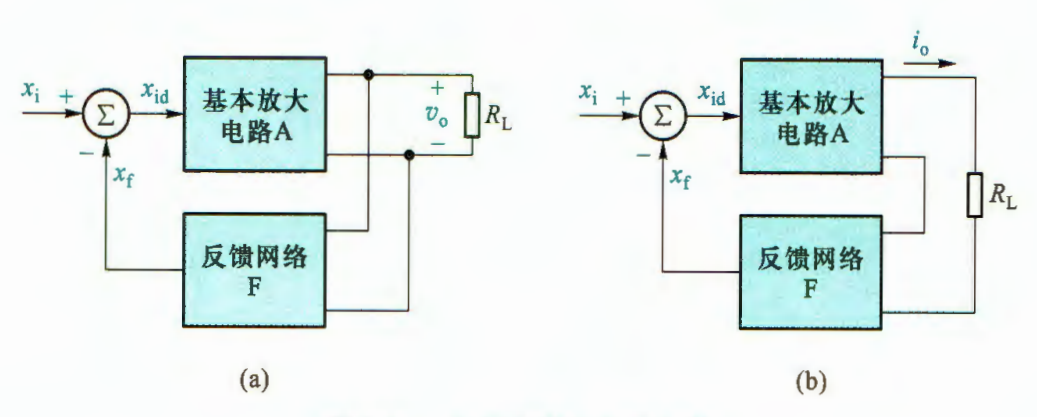
\includegraphics[width=0.75\linewidth]{pic/电压反馈和电流反馈.png}
    \caption{电压反馈和电流反馈(a)电压反馈(b)电流反馈\cite{康华光}\label{电压反馈和电流反馈}}
\end{figure}

此外,反馈信号取自于谁,就可以稳定谁。电压负反馈可以稳定输出电压,电流负反馈可以稳定输出电流。

\subsection{四种组态的负反馈放大电路}
由上述两种分类进行两两组合,就可以得到四种组态的放大电路,即电压串联、电流串联、电压并联、电流并联。

在实际中,往往会根据不同的需求来决定采用哪种放大电路。电路中究竟应该引入串联反馈还是并联反馈,取决于输入信号是恒压源还是恒流源;而应该引入电压反馈还是电流反馈,取决于负载需要的是稳定的电压信号还是电流信号。

\subsection{负反馈放大电路增益的一般表达式}
负反馈放大电路组成的框图如图\ref{负反馈放大电路的组成框图}所示。

\begin{figure}[htb]
    \centering
    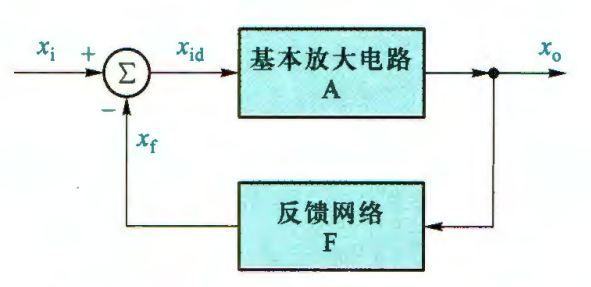
\includegraphics[width=0.5\linewidth]{pic/负反馈放大电路的组成框图.png}
    \caption{负反馈放大电路的组成框图\cite{康华光}\label{负反馈放大电路的组成框图}}
\end{figure}

其中$x_{\mathrm{i}}$表示输入信号,$x_{\mathrm{o}}$表示输出信号,$x_{\mathrm{id}}=x_{\mathrm{i}}-x_{\mathrm{f}}$表示净输入信号,$x_{\mathrm{f}}$表示反馈信号。

\textbf{基本放大电路增益(开环增益)}为$A=x_{\mathrm{o}}/x_{\mathrm{id}}$,\textbf{反馈系数}$F=x_{\mathrm{f}}/x_{\mathrm{o}}$,而\textbf{负反馈放大电路的增益(闭环增益)}为$A_{\mathrm{f}}=x_{\mathrm{o}}/x_{\mathrm{i}}$。

则可以得到闭环增益的一般表达式
\begin{equation}\label{闭环增益}
    A_{\mathrm{f}}=\frac{Ax_{\mathrm{id}}}{x_{\mathrm{id}}+AFx_{\mathrm{id}}}=\frac{A}{1+AF},
\end{equation}

其中,$AF$被称为\textbf{环路增益}\index{H!环路增益},$(1+AF)$被称为\textbf{反馈深度}\index{F!反馈!反馈深度}。可以看到,引⼊负反馈后电路增益降低,倍数与反馈深度有关。

\subsection{负反馈对放大电路性能的影响}

\subsubsection{一、提高增益的稳定性}
根据计算可以得到
\begin{equation}
    \frac{\mathrm{d}A_{\mathrm{f}}}{A_{\mathrm{f}}}=\frac{1}{1+AF}\frac{\mathrm{d}A}{A}
\end{equation}

可见,$A_{\mathrm{f}}$的稳定性是$A$的$(1+AF)$倍。

\subsubsection{二、对输入输出电阻的影响}
1.串联负反馈增大输入电阻:$R_\mathrm{if}=(1+AF)R_\mathrm{i}$。

2.并联负反馈减小输入电阻:$R_\mathrm{if}=R_\mathrm{i}/(1+AF)$。

3.电压负反馈减小输出电阻:$R_\mathrm{of}=R_\mathrm{o}/(1+AF)$。

4.电流负反馈增大输出电阻:$R_\mathrm{of}=(1+AF)R_\mathrm{o}$。

\subsubsection{三、减小非线性失真}

\subsubsection{四、抑制反馈环内噪声}

\subsubsection{五、扩展带宽}

虽然引入负反馈减小了增益,但整体来说,负反馈是利大于弊的。

\begin{figure}[htb]
    \centering
    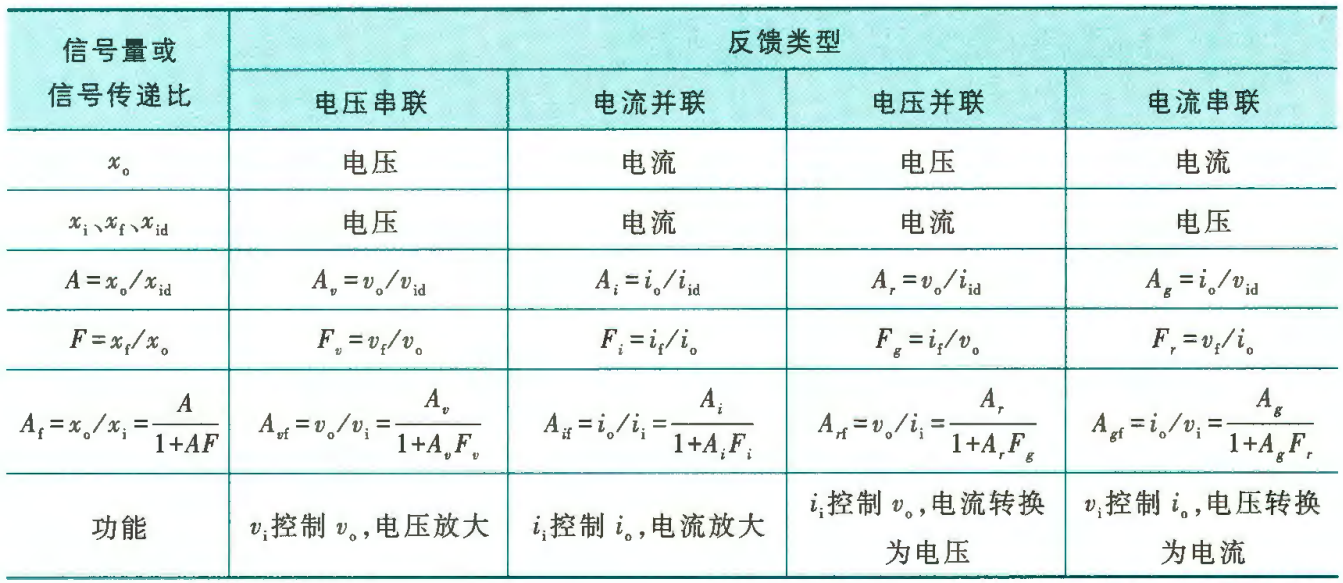
\includegraphics[width=0.99\linewidth]{pic/负反馈放大电路中各种信号量的含义.png}
    \caption{负反馈放大电路中各种信号量的含义\cite{康华光}\label{负反馈放大电路中各种信号量的含义}}
\end{figure}

\section{深度负反馈}
当$(1+AF)\gg 1$时,称为\textbf{深度负反馈}\index{F!反馈!深度负反馈},此时
\begin{equation}
    A_{\mathrm{f}}=\frac{1}{F},
\end{equation}

可以看到,闭环增益只取决于反馈系数,与开环增益无关。本质上,深度负反馈是将\ref{闭环增益}中分母上的净输入量$x_{\mathrm{id}}$忽略了。

无论是串联反馈还是并联反馈,只要在深度负反馈的条件下,均有$v_{\mathrm{id}}=0$(虚短)和$i_{\mathrm{id}}=0$(虚断)同时存在。利用这两个性质可以很方便地求出负反馈电路的闭环增益。